% Created by tikzDevice version 0.12.6 on 2024-06-05 05:34:51
% !TEX encoding = UTF-8 Unicode
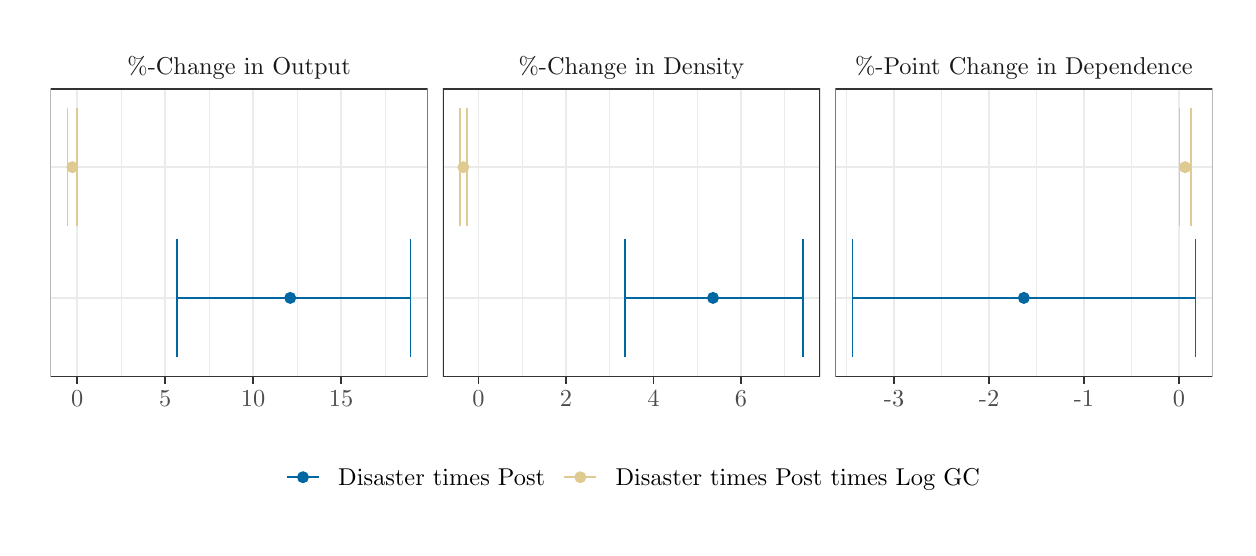
\begin{tikzpicture}[x=1pt,y=1pt]
\definecolor{fillColor}{RGB}{255,255,255}
\path[use as bounding box,fill=fillColor,fill opacity=0.00] (0,0) rectangle (433.62,180.67);
\begin{scope}
\path[clip] (  0.00,  0.00) rectangle (433.62,180.67);
\definecolor{drawColor}{RGB}{255,255,255}
\definecolor{fillColor}{RGB}{255,255,255}

\path[draw=drawColor,line width= 0.6pt,line join=round,line cap=round,fill=fillColor] (  0.00,  0.00) rectangle (433.62,180.68);
\end{scope}
\begin{scope}
\path[clip] (  8.25, 54.68) rectangle (144.54,158.60);
\definecolor{fillColor}{RGB}{255,255,255}

\path[fill=fillColor] (  8.25, 54.68) rectangle (144.54,158.60);
\definecolor{drawColor}{gray}{0.92}

\path[draw=drawColor,line width= 0.3pt,line join=round] ( 33.80, 54.68) --
	( 33.80,158.60);

\path[draw=drawColor,line width= 0.3pt,line join=round] ( 65.59, 54.68) --
	( 65.59,158.60);

\path[draw=drawColor,line width= 0.3pt,line join=round] ( 97.37, 54.68) --
	( 97.37,158.60);

\path[draw=drawColor,line width= 0.3pt,line join=round] (129.16, 54.68) --
	(129.16,158.60);

\path[draw=drawColor,line width= 0.6pt,line join=round] (  8.25, 83.02) --
	(144.54, 83.02);

\path[draw=drawColor,line width= 0.6pt,line join=round] (  8.25,130.26) --
	(144.54,130.26);

\path[draw=drawColor,line width= 0.6pt,line join=round] ( 17.91, 54.68) --
	( 17.91,158.60);

\path[draw=drawColor,line width= 0.6pt,line join=round] ( 49.69, 54.68) --
	( 49.69,158.60);

\path[draw=drawColor,line width= 0.6pt,line join=round] ( 81.48, 54.68) --
	( 81.48,158.60);

\path[draw=drawColor,line width= 0.6pt,line join=round] (113.27, 54.68) --
	(113.27,158.60);
\definecolor{drawColor}{RGB}{0,103,162}
\definecolor{fillColor}{RGB}{0,103,162}

\path[draw=drawColor,line width= 0.4pt,line join=round,line cap=round,fill=fillColor] ( 94.87, 83.02) circle (  1.96);
\definecolor{drawColor}{RGB}{223,203,145}
\definecolor{fillColor}{RGB}{223,203,145}

\path[draw=drawColor,line width= 0.4pt,line join=round,line cap=round,fill=fillColor] ( 16.14,130.26) circle (  1.96);
\definecolor{drawColor}{RGB}{0,103,162}

\path[draw=drawColor,line width= 0.6pt,line join=round] (138.34, 61.76) --
	(138.34,104.28);

\path[draw=drawColor,line width= 0.6pt,line join=round] (138.34, 83.02) --
	( 53.90, 83.02);

\path[draw=drawColor,line width= 0.6pt,line join=round] ( 53.90, 61.76) --
	( 53.90,104.28);
\definecolor{drawColor}{RGB}{223,203,145}

\path[draw=drawColor,line width= 0.6pt,line join=round] ( 17.84,109.00) --
	( 17.84,151.52);

\path[draw=drawColor,line width= 0.6pt,line join=round] ( 17.84,130.26) --
	( 14.45,130.26);

\path[draw=drawColor,line width= 0.6pt,line join=round] ( 14.45,109.00) --
	( 14.45,151.52);
\definecolor{drawColor}{gray}{0.20}

\path[draw=drawColor,line width= 0.6pt,line join=round,line cap=round] (  8.25, 54.68) rectangle (144.54,158.60);
\end{scope}
\begin{scope}
\path[clip] (150.04, 54.68) rectangle (286.33,158.60);
\definecolor{fillColor}{RGB}{255,255,255}

\path[fill=fillColor] (150.04, 54.68) rectangle (286.33,158.60);
\definecolor{drawColor}{gray}{0.92}

\path[draw=drawColor,line width= 0.3pt,line join=round] (178.69, 54.68) --
	(178.69,158.60);

\path[draw=drawColor,line width= 0.3pt,line join=round] (210.30, 54.68) --
	(210.30,158.60);

\path[draw=drawColor,line width= 0.3pt,line join=round] (241.91, 54.68) --
	(241.91,158.60);

\path[draw=drawColor,line width= 0.3pt,line join=round] (273.51, 54.68) --
	(273.51,158.60);

\path[draw=drawColor,line width= 0.6pt,line join=round] (150.04, 83.02) --
	(286.33, 83.02);

\path[draw=drawColor,line width= 0.6pt,line join=round] (150.04,130.26) --
	(286.33,130.26);

\path[draw=drawColor,line width= 0.6pt,line join=round] (162.89, 54.68) --
	(162.89,158.60);

\path[draw=drawColor,line width= 0.6pt,line join=round] (194.50, 54.68) --
	(194.50,158.60);

\path[draw=drawColor,line width= 0.6pt,line join=round] (226.10, 54.68) --
	(226.10,158.60);

\path[draw=drawColor,line width= 0.6pt,line join=round] (257.71, 54.68) --
	(257.71,158.60);
\definecolor{drawColor}{RGB}{0,103,162}
\definecolor{fillColor}{RGB}{0,103,162}

\path[draw=drawColor,line width= 0.4pt,line join=round,line cap=round,fill=fillColor] (247.65, 83.02) circle (  1.96);
\definecolor{drawColor}{RGB}{223,203,145}
\definecolor{fillColor}{RGB}{223,203,145}

\path[draw=drawColor,line width= 0.4pt,line join=round,line cap=round,fill=fillColor] (157.44,130.26) circle (  1.96);
\definecolor{drawColor}{RGB}{0,103,162}

\path[draw=drawColor,line width= 0.6pt,line join=round] (280.13, 61.76) --
	(280.13,104.28);

\path[draw=drawColor,line width= 0.6pt,line join=round] (280.13, 83.02) --
	(215.78, 83.02);

\path[draw=drawColor,line width= 0.6pt,line join=round] (215.78, 61.76) --
	(215.78,104.28);
\definecolor{drawColor}{RGB}{223,203,145}

\path[draw=drawColor,line width= 0.6pt,line join=round] (158.65,109.00) --
	(158.65,151.52);

\path[draw=drawColor,line width= 0.6pt,line join=round] (158.65,130.26) --
	(156.24,130.26);

\path[draw=drawColor,line width= 0.6pt,line join=round] (156.24,109.00) --
	(156.24,151.52);
\definecolor{drawColor}{gray}{0.20}

\path[draw=drawColor,line width= 0.6pt,line join=round,line cap=round] (150.04, 54.68) rectangle (286.33,158.60);
\end{scope}
\begin{scope}
\path[clip] (291.83, 54.68) rectangle (428.12,158.60);
\definecolor{fillColor}{RGB}{255,255,255}

\path[fill=fillColor] (291.83, 54.68) rectangle (428.12,158.60);
\definecolor{drawColor}{gray}{0.92}

\path[draw=drawColor,line width= 0.3pt,line join=round] (295.94, 54.68) --
	(295.94,158.60);

\path[draw=drawColor,line width= 0.3pt,line join=round] (330.24, 54.68) --
	(330.24,158.60);

\path[draw=drawColor,line width= 0.3pt,line join=round] (364.54, 54.68) --
	(364.54,158.60);

\path[draw=drawColor,line width= 0.3pt,line join=round] (398.84, 54.68) --
	(398.84,158.60);

\path[draw=drawColor,line width= 0.6pt,line join=round] (291.83, 83.02) --
	(428.12, 83.02);

\path[draw=drawColor,line width= 0.6pt,line join=round] (291.83,130.26) --
	(428.12,130.26);

\path[draw=drawColor,line width= 0.6pt,line join=round] (313.09, 54.68) --
	(313.09,158.60);

\path[draw=drawColor,line width= 0.6pt,line join=round] (347.39, 54.68) --
	(347.39,158.60);

\path[draw=drawColor,line width= 0.6pt,line join=round] (381.69, 54.68) --
	(381.69,158.60);

\path[draw=drawColor,line width= 0.6pt,line join=round] (415.99, 54.68) --
	(415.99,158.60);
\definecolor{drawColor}{RGB}{0,103,162}
\definecolor{fillColor}{RGB}{0,103,162}

\path[draw=drawColor,line width= 0.4pt,line join=round,line cap=round,fill=fillColor] (359.97, 83.02) circle (  1.96);
\definecolor{drawColor}{RGB}{223,203,145}
\definecolor{fillColor}{RGB}{223,203,145}

\path[draw=drawColor,line width= 0.4pt,line join=round,line cap=round,fill=fillColor] (418.23,130.26) circle (  1.96);
\definecolor{drawColor}{RGB}{0,103,162}

\path[draw=drawColor,line width= 0.6pt,line join=round] (421.93, 61.76) --
	(421.93,104.28);

\path[draw=drawColor,line width= 0.6pt,line join=round] (421.93, 83.02) --
	(298.02, 83.02);

\path[draw=drawColor,line width= 0.6pt,line join=round] (298.02, 61.76) --
	(298.02,104.28);
\definecolor{drawColor}{RGB}{223,203,145}

\path[draw=drawColor,line width= 0.6pt,line join=round] (420.29,109.00) --
	(420.29,151.52);

\path[draw=drawColor,line width= 0.6pt,line join=round] (420.29,130.26) --
	(416.17,130.26);

\path[draw=drawColor,line width= 0.6pt,line join=round] (416.17,109.00) --
	(416.17,151.52);
\definecolor{drawColor}{gray}{0.20}

\path[draw=drawColor,line width= 0.6pt,line join=round,line cap=round] (291.83, 54.68) rectangle (428.12,158.60);
\end{scope}
\begin{scope}
\path[clip] (  8.25,158.60) rectangle (144.54,175.17);
\definecolor{drawColor}{gray}{0.10}

\node[text=drawColor,anchor=base,inner sep=0pt, outer sep=0pt, scale=  0.88] at ( 76.40,163.86) {\%-Change in Output};
\end{scope}
\begin{scope}
\path[clip] (150.04,158.60) rectangle (286.33,175.17);
\definecolor{drawColor}{gray}{0.10}

\node[text=drawColor,anchor=base,inner sep=0pt, outer sep=0pt, scale=  0.88] at (218.18,163.86) {\%-Change in Density};
\end{scope}
\begin{scope}
\path[clip] (291.83,158.60) rectangle (428.12,175.17);
\definecolor{drawColor}{gray}{0.10}

\node[text=drawColor,anchor=base,inner sep=0pt, outer sep=0pt, scale=  0.88] at (359.98,163.86) {\%-Point Change in Dependence};
\end{scope}
\begin{scope}
\path[clip] (  0.00,  0.00) rectangle (433.62,180.67);
\definecolor{drawColor}{gray}{0.20}

\path[draw=drawColor,line width= 0.6pt,line join=round] ( 17.91, 51.93) --
	( 17.91, 54.68);

\path[draw=drawColor,line width= 0.6pt,line join=round] ( 49.69, 51.93) --
	( 49.69, 54.68);

\path[draw=drawColor,line width= 0.6pt,line join=round] ( 81.48, 51.93) --
	( 81.48, 54.68);

\path[draw=drawColor,line width= 0.6pt,line join=round] (113.27, 51.93) --
	(113.27, 54.68);
\end{scope}
\begin{scope}
\path[clip] (  0.00,  0.00) rectangle (433.62,180.67);
\definecolor{drawColor}{gray}{0.30}

\node[text=drawColor,anchor=base,inner sep=0pt, outer sep=0pt, scale=  0.88] at ( 17.91, 43.66) {0};

\node[text=drawColor,anchor=base,inner sep=0pt, outer sep=0pt, scale=  0.88] at ( 49.69, 43.66) {5};

\node[text=drawColor,anchor=base,inner sep=0pt, outer sep=0pt, scale=  0.88] at ( 81.48, 43.66) {10};

\node[text=drawColor,anchor=base,inner sep=0pt, outer sep=0pt, scale=  0.88] at (113.27, 43.66) {15};
\end{scope}
\begin{scope}
\path[clip] (  0.00,  0.00) rectangle (433.62,180.67);
\definecolor{drawColor}{gray}{0.20}

\path[draw=drawColor,line width= 0.6pt,line join=round] (162.89, 51.93) --
	(162.89, 54.68);

\path[draw=drawColor,line width= 0.6pt,line join=round] (194.50, 51.93) --
	(194.50, 54.68);

\path[draw=drawColor,line width= 0.6pt,line join=round] (226.10, 51.93) --
	(226.10, 54.68);

\path[draw=drawColor,line width= 0.6pt,line join=round] (257.71, 51.93) --
	(257.71, 54.68);
\end{scope}
\begin{scope}
\path[clip] (  0.00,  0.00) rectangle (433.62,180.67);
\definecolor{drawColor}{gray}{0.30}

\node[text=drawColor,anchor=base,inner sep=0pt, outer sep=0pt, scale=  0.88] at (162.89, 43.66) {0};

\node[text=drawColor,anchor=base,inner sep=0pt, outer sep=0pt, scale=  0.88] at (194.50, 43.66) {2};

\node[text=drawColor,anchor=base,inner sep=0pt, outer sep=0pt, scale=  0.88] at (226.10, 43.66) {4};

\node[text=drawColor,anchor=base,inner sep=0pt, outer sep=0pt, scale=  0.88] at (257.71, 43.66) {6};
\end{scope}
\begin{scope}
\path[clip] (  0.00,  0.00) rectangle (433.62,180.67);
\definecolor{drawColor}{gray}{0.20}

\path[draw=drawColor,line width= 0.6pt,line join=round] (313.09, 51.93) --
	(313.09, 54.68);

\path[draw=drawColor,line width= 0.6pt,line join=round] (347.39, 51.93) --
	(347.39, 54.68);

\path[draw=drawColor,line width= 0.6pt,line join=round] (381.69, 51.93) --
	(381.69, 54.68);

\path[draw=drawColor,line width= 0.6pt,line join=round] (415.99, 51.93) --
	(415.99, 54.68);
\end{scope}
\begin{scope}
\path[clip] (  0.00,  0.00) rectangle (433.62,180.67);
\definecolor{drawColor}{gray}{0.30}

\node[text=drawColor,anchor=base,inner sep=0pt, outer sep=0pt, scale=  0.88] at (313.09, 43.66) {-3};

\node[text=drawColor,anchor=base,inner sep=0pt, outer sep=0pt, scale=  0.88] at (347.39, 43.66) {-2};

\node[text=drawColor,anchor=base,inner sep=0pt, outer sep=0pt, scale=  0.88] at (381.69, 43.66) {-1};

\node[text=drawColor,anchor=base,inner sep=0pt, outer sep=0pt, scale=  0.88] at (415.99, 43.66) {0};
\end{scope}
\begin{scope}
\path[clip] (  0.00,  0.00) rectangle (433.62,180.67);
\definecolor{fillColor}{RGB}{255,255,255}

\path[fill=fillColor] ( 86.76,  5.50) rectangle (349.61, 30.95);
\end{scope}
\begin{scope}
\path[clip] (  0.00,  0.00) rectangle (433.62,180.67);
\definecolor{fillColor}{RGB}{255,255,255}

\path[fill=fillColor] ( 92.26, 11.00) rectangle (106.71, 25.45);
\end{scope}
\begin{scope}
\path[clip] (  0.00,  0.00) rectangle (433.62,180.67);
\definecolor{drawColor}{RGB}{0,103,162}
\definecolor{fillColor}{RGB}{0,103,162}

\path[draw=drawColor,line width= 0.4pt,line join=round,line cap=round,fill=fillColor] ( 99.49, 18.23) circle (  1.96);
\end{scope}
\begin{scope}
\path[clip] (  0.00,  0.00) rectangle (433.62,180.67);
\definecolor{drawColor}{RGB}{0,103,162}

\path[draw=drawColor,line width= 0.6pt,line join=round] ( 93.70, 18.23) -- (105.27, 18.23);
\end{scope}
\begin{scope}
\path[clip] (  0.00,  0.00) rectangle (433.62,180.67);
\definecolor{fillColor}{RGB}{255,255,255}

\path[fill=fillColor] (192.47, 11.00) rectangle (206.92, 25.45);
\end{scope}
\begin{scope}
\path[clip] (  0.00,  0.00) rectangle (433.62,180.67);
\definecolor{drawColor}{RGB}{223,203,145}
\definecolor{fillColor}{RGB}{223,203,145}

\path[draw=drawColor,line width= 0.4pt,line join=round,line cap=round,fill=fillColor] (199.70, 18.23) circle (  1.96);
\end{scope}
\begin{scope}
\path[clip] (  0.00,  0.00) rectangle (433.62,180.67);
\definecolor{drawColor}{RGB}{223,203,145}

\path[draw=drawColor,line width= 0.6pt,line join=round] (193.92, 18.23) -- (205.48, 18.23);
\end{scope}
\begin{scope}
\path[clip] (  0.00,  0.00) rectangle (433.62,180.67);
\definecolor{drawColor}{RGB}{0,0,0}

\node[text=drawColor,anchor=base west,inner sep=0pt, outer sep=0pt, scale=  0.88] at (112.21, 15.20) {Disaster times Post};
\end{scope}
\begin{scope}
\path[clip] (  0.00,  0.00) rectangle (433.62,180.67);
\definecolor{drawColor}{RGB}{0,0,0}

\node[text=drawColor,anchor=base west,inner sep=0pt, outer sep=0pt, scale=  0.88] at (212.42, 15.20) {Disaster times Post times Log GC};
\end{scope}
\end{tikzpicture}
